\documentclass[12pt]{ctexart}%中文包
\usepackage{graphicx}%图片引用包
\usepackage{amssymb}%特殊符号
\usepackage{amsmath,amsfonts,bm}%矩阵
\usepackage{amsthm}%定理
\usepackage{geometry}%缩放
\usepackage{hyperref}%超链接
\usepackage{framed}%框框
\usepackage{color}%颜色
\usepackage{mathrsfs}%花体
\usepackage{anyfontsize}
\usepackage{indentfirst}%缩进
\usepackage{extsizes}%size
\usepackage{newtxtext,newtxmath}%times风格字体
\usepackage{mdframed}%边栏

\surroundwithmdframed[
  linecolor=gray,
  topline=false,
  bottomline=false,
  rightline=false,
  linewidth=4pt,
  innerleftmargin=10pt,
  innerrightmargin=10pt,
  innertopmargin=0pt,
  innerbottommargin=10pt
]{theorem}
\surroundwithmdframed[
    linecolor=black,
    leftline=false,
    rightline=false,
    linewidth=0.5pt,
    innerleftmargin=10pt,
    innerrightmargin=10pt,
    innertopmargin=0pt,
    innerbottommargin=10pt
]{note}

\newtheorem{theorem}{Law}
\newtheorem{note}{Note}



\geometry{a4paper,scale=0.85}
\hypersetup
    {
        hypertex=true,
        colorlinks=true,
        linkcolor=blue,
        anchorcolor=blue,
        citecolor=blue
    }


\title{Geometrical Optics\\几何光学}

\author{Jerry Ling} 

\date{\today}
 
\begin{document}  %begin后括号内是文件类型
\maketitle  %生成标题
上一篇笔记中讨论了作为波的光的基本形式,也介绍了导出波前的惠更斯原理和光线最短路径传播的费马原理。本篇我们将重点放在\textbf{近轴(coaxial)系统}的研究中。该系统中不同界面的入射角度接近0度,因而斯涅尔定律简化为如下形式:
\begin{theorem}[Snell's Law in Coaxial System]\label{snell}
    \[n_1\theta_1=n_2\theta_2\]
\end{theorem}
定律\ref{snell}将极大简化对光学系统的分析,因为其将之简化为一个线性的问题。另外,为了避免混淆,接下来的讨论中我们规定零点左边的坐标为负;向左边凸起的半径/曲率为正;光线总是由左边射入右边。
\section*{单个透镜在空气中的成像}
\begin{figure}[t] %two figures
        \centering
        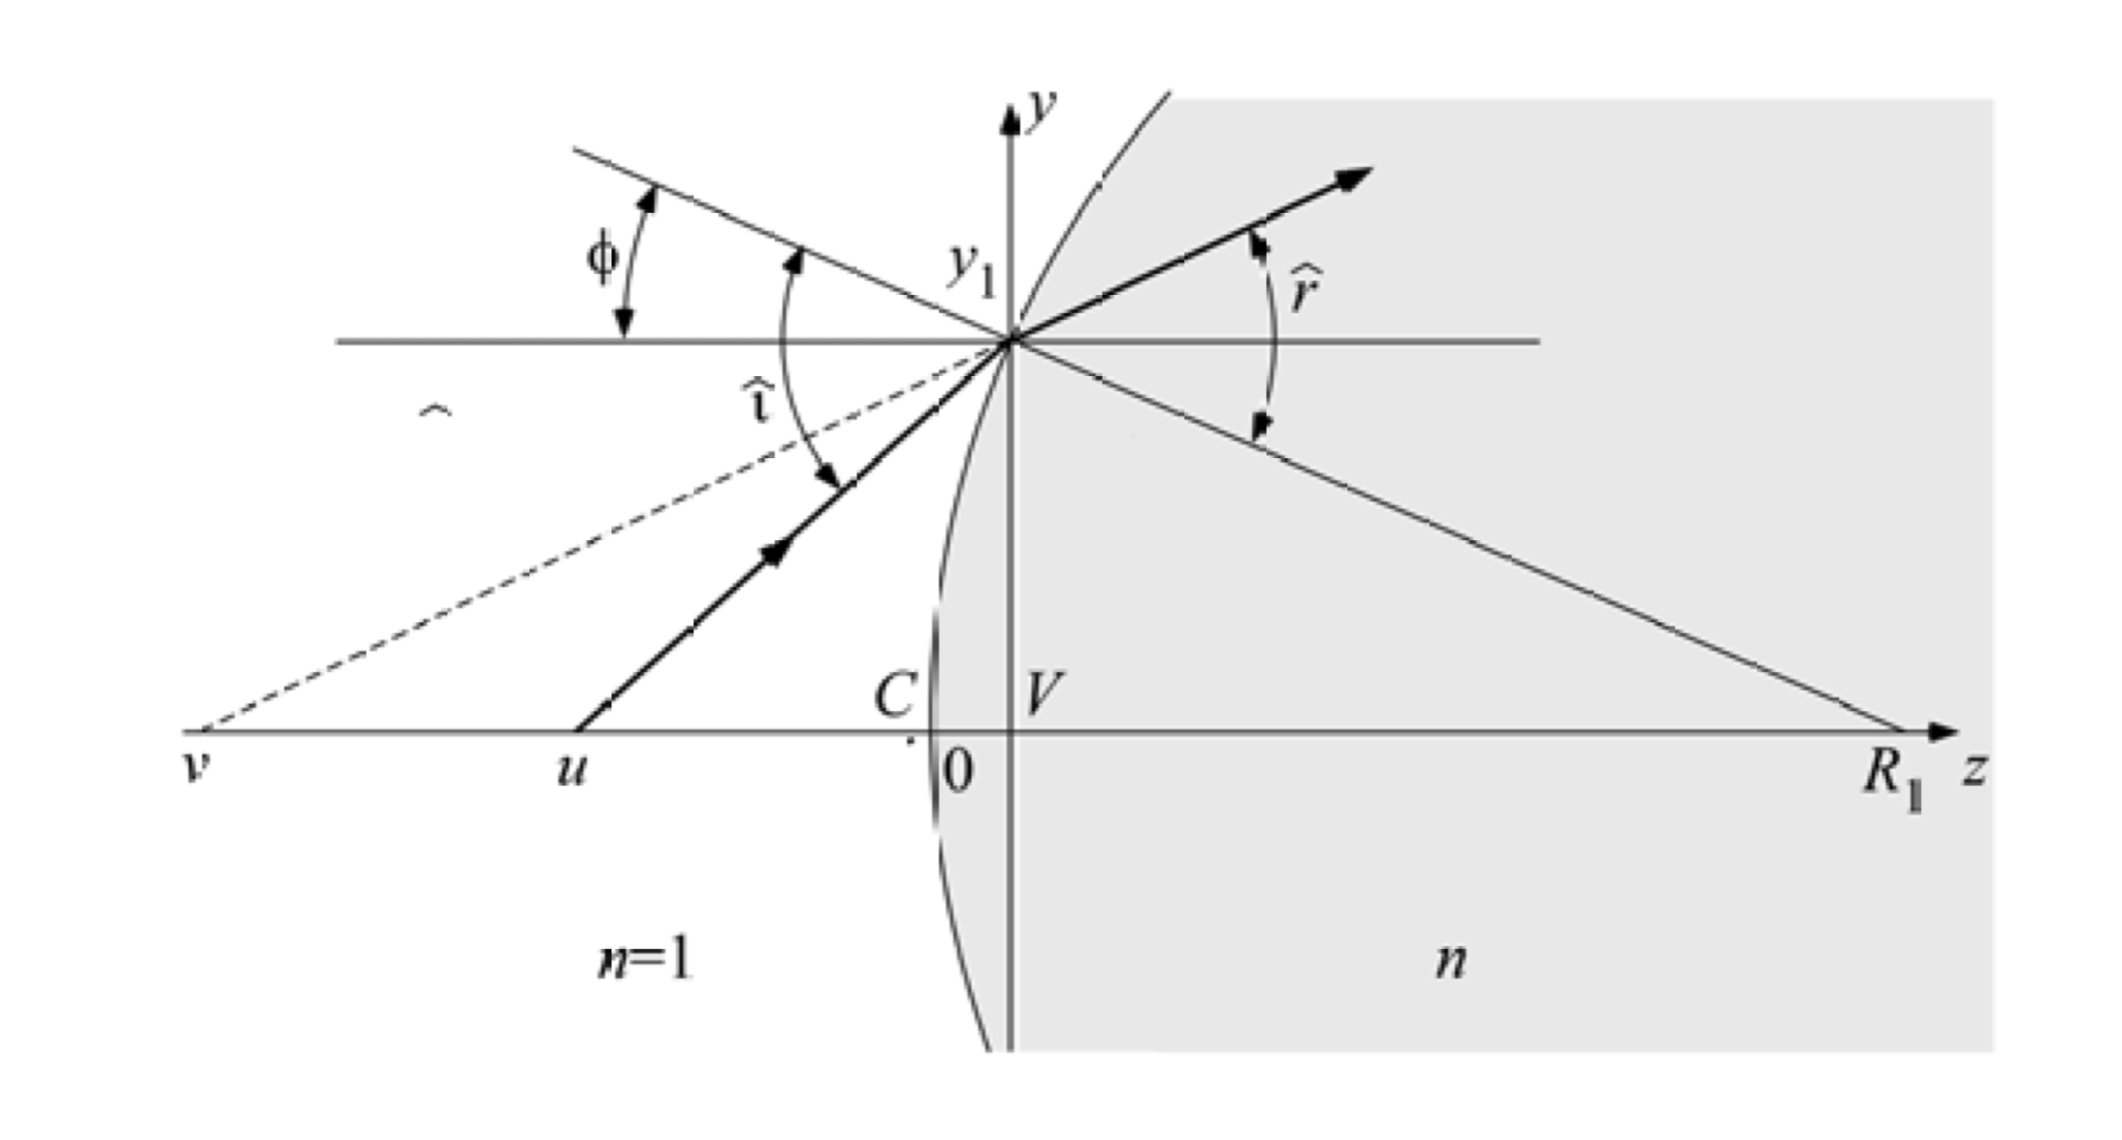
\includegraphics[width=0.8\textwidth]{Image/2_single_lens.png}
        \caption{Geometric of Refraction}
        \label{single_lens_1}
\end{figure}
考虑一个半径为R1的球面,界面近似位于0点。按照图\ref{single_lens_1}的几何关系和定律\ref{snell}可以得到:
\begin{equation}
    -\frac{n}{v}+\frac{1}{u}=\frac{1}{R_1}(1-n)
\end{equation}
其中u是物距(负数),v是u经过界面后折射的虚像位置。再考虑另一个半径为R2(负数)的球面,界面同样近似在0点,与前者构成一个凸透镜。那么上式中的v可以作为新的物距代入自身;折射率显然也变成1/n:
\begin{equation}
    -\frac{1/n}{v'}+\frac{1}{v}=\frac{1}{R_2}(1-1/n)
\end{equation}
v'是新的像距。连立两式得到:
\begin{equation}
    -\frac{1}{u}+\frac{1}{v}=(n-1)(\frac{1}{R_1}-\frac{1}{R_2})
    \label{f}
\end{equation}
定义右半边表达式为1/f,则得到透镜公式:
\begin{theorem}[Lens Makers' Equation]\label{lens}
    \[-\frac{1}{u}+\frac{1}{v}=\frac{1}{f}\]
\end{theorem}
\par 注意该公式的使用条件为凸面半径远远大于入射高度,即透镜应为\textbf{薄透镜(thin lens)}。f称为\textbf{焦距(focal length)},1/f称为\textbf{power of lens};焦距为负数的薄透镜称为\textbf{diverging lens}。过距离原点长度为焦距的两个点(F1,F2)与轴的垂面称为\textbf{焦平面(focal plane)}。取轴上一点u以角度$\theta$入射,其像为v。则入射高度为$y=-u\theta$,从像发出的光同焦平面的交点高度为$d=\frac{y}{-v}(-v+f)$。则代入透镜公式得到:
\begin{equation}
    d=\theta f
\end{equation}
换言之,任何以角度$\theta$入射薄透镜的光都汇聚在焦平面上高度为$d=\theta f$的一点上。因为u接近零点时v也接近零,即等效于没有改变位置,故任何透过中心的光线都不发生折射。最后,因为u趋向无限时v=f,所以平行于轴的入射光过焦点F1。根据这三条法则,即可用尺规作图来对任何点光源进行\textbf{光线追踪(Ray Tracing)}。
\begin{note}[Fresnel lens]
    菲涅尔透镜实质上保留了圆弧表面的弧度而舍弃了光滑性。通过切割的方法可以制造重量很轻的薄透镜用于大型聚光或投影装置。但由于反射和散射的增加不适合用于高分辨的成像。
\end{note}
\section*{简单放大镜}
首先考虑一个用于放大物像的凸透镜。在几何光学中,物体上的每一点发出的光通过透镜汇聚在某点即称为成像,当物体没有厚度时可定义相互\textbf{共轭}的物平面和像平面。人眼的晶状体通过变厚来使近处的非平行光线汇聚到视网膜上,而能够聚焦的最近距离称为人眼的\textbf{近点(near point)},见图\ref{single_lens_2}“eyes”图。当使用凸透镜后,焦距内物体不成实像,而是在后方成一个较大的虚像,可将像搬到近点以外,见图\ref{single_lens_2}前两副图。
\par 观察蓝色\textbf{主射线(chief ray)}(顶点向透镜中心)。不难发现,在晶状体调节范围内,视网膜成像大小同该射线入射角度$\varphi$正比。因而定义\textbf{magnifying power}或\textbf{角放大率(angular magnification,$M_A$)}为放大后主射线角度与近点处主射线角度之比,或放大后视网膜上像线性大小与近点处物体在视网膜上像线性大小之比。设凸透镜离眼距离$l$,近点距眼$D$,物高$h_0$,像高$h_I$;放大和近点入射角度分别为$\varphi$和$\varphi_0$。可列:
\begin{figure}[t] %two figures
    \centering
    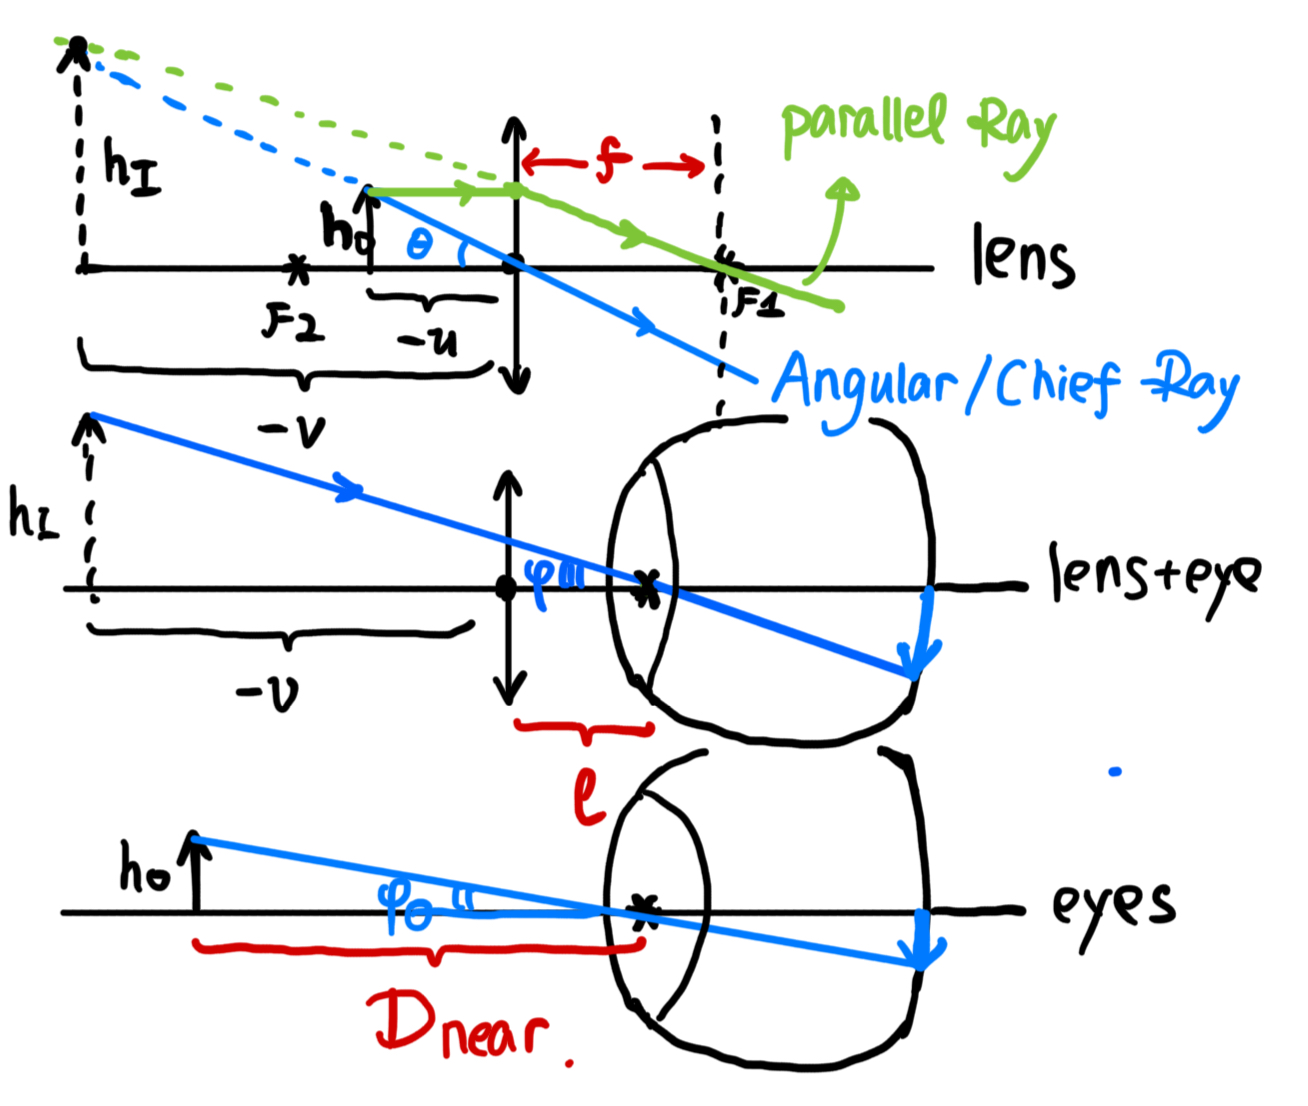
\includegraphics[width=0.6\textwidth]{Image/2_lens_ray.jpg}
    \caption{Lens Ray Tracing}
    \label{single_lens_2}
\end{figure}

\begin{equation}
    \varphi=\frac{h_I}{-v+l}
\end{equation}
\begin{equation}
    \varphi_0=\frac{h_0}{D}
\end{equation}
其中透镜成虚像高$h_I$和实像高$h_0$比例为v/u。简化后得到:
\begin{framed}
    \begin{equation}
        M_{A}=\varphi/\varphi_0=\frac{D}{f}*\frac{f-v}{l-v}
    \end{equation}
\end{framed}
\noindent 取l=0,放大率最大化(-v take min),则v=D,$M_A=1+D/f$。取v为负无穷,即物距u=-f,则$M_A=D/f$。
\section*{简单镜片组系统}
\subsection*{光阑,光瞳和重要射线}
多个透镜可实现更多功能。为方便讨论,考虑两条重要的射线。近轴系统只对光线的角度和高度进行线性变换,因而通过设置高度为0的射线即可直观得到系统对角度的操作。由于透镜尺寸有限,轴上(on-axis)光源的入射角度将存在最大值。称限制体系总光线进量(即O点射线的角度)的实体为\textbf{孔径光阑(aperture stop, A.S.)},O点出发过其边沿的光线为\textbf{边沿射线(marginal ray)},见图\ref{pupil}蓝色线(L1是孔径光阑)。易见O点的射线最大智能以$\alpha$角度入射,角放大率$\beta/\alpha$。在不确定A.S.时候可不断增加角度来判断充当之的部件。
\par 因0角度的射线包含信息太少,另一条射线并不设为0角度,而是希望有一条独立于孔径光阑大小的射线。显然,过A.S.中心的射线满足该要求,称为\textbf{主射线(chief ray)}。同样,由于有限性,主射线角度也存在最大值。称限制视野大小的实体为\textbf{视场光阑(field stop, F.S.)},过起边沿的主射线为图\ref{pupil}中绿色线。F.S.可用相似方法确认。注意,边沿射线的角度仅和亮度相关,而主射线的角度直接\textbf{限制视角(field of view)}。
\par \textbf{光瞳(pupils)}是A.S.的像。图\ref{pupil}中入射光瞳即A.S.本身,而出射光瞳是其关于后续透镜L2的像。注意到主射线汇聚在L1的像位置,故用两条线即可判断入射(如前方还有透镜可进行类似光线追踪)和出射光瞳位置。事实上,这两条射线完全定义任一近轴光学系统。
\subsection*{望远镜和显微镜}
\begin{figure}[t] %two figures
    \centering
    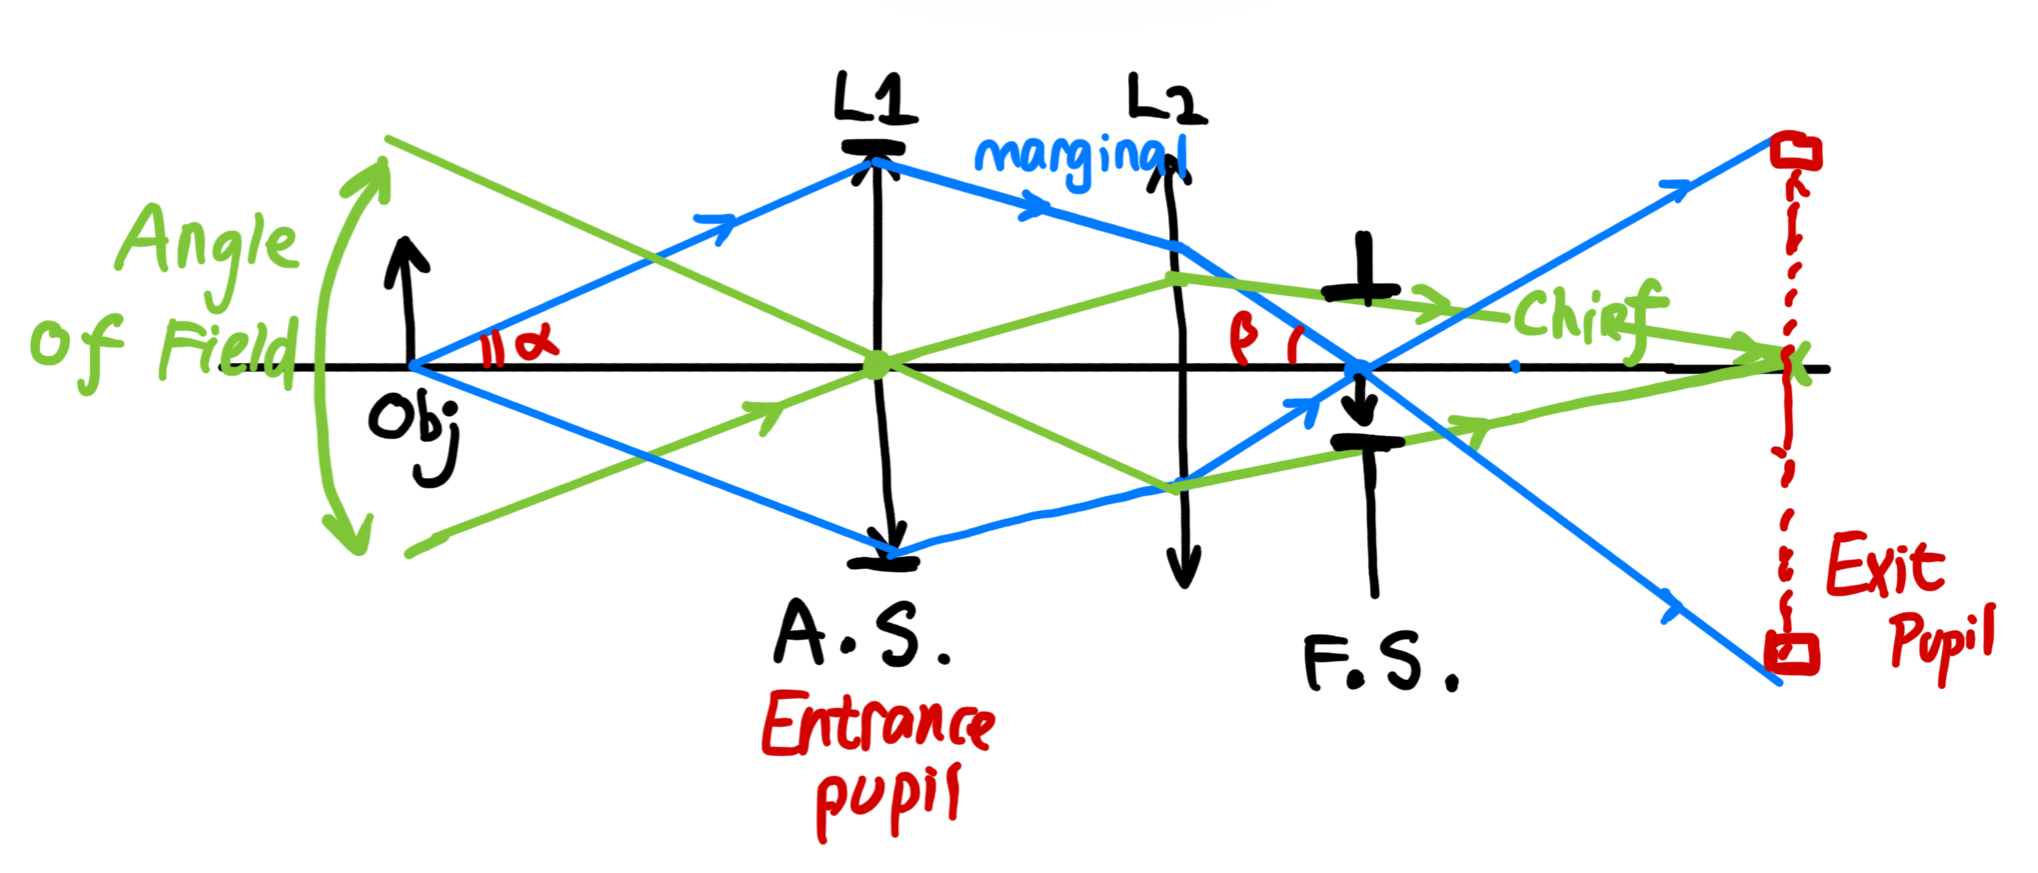
\includegraphics[width=0.8\textwidth]{Image/2_pupil.jpeg}
    \caption{Rays, Stops and Pupils}
    \label{pupil}
\end{figure}
\par 望远镜(telescope)系统能将一束角度为$\alpha$的平行光放大为角度为$\beta$的平行光。其实现利用两个焦点重合点凸透镜,见图\ref{telescope}。由于远处物体近似于平行光,角放大率(放大前后角度比)是我们关心的参数:
\begin{equation}
    M_A=\frac{f_1}{f_2}
\end{equation}
远处的物体仍在无穷远处成虚像,或亦可理解为L1成的实像被放大镜L2成虚像(见上节)。
\par 注意,当L2孔径较小时,离轴较远的点光源(F平面上的实像上部)进入L2的角度很小,其像在离轴方向将逐渐变暗。该现象称为\textbf{晕影(vignetting)}(图\ref{telescope}上)。减少晕影的方法之一是在F处设一人为的孔径使之小于L2尺寸(图\ref{telescope}下)。由于焦平面F上成实像,新的孔径充当F.S.。进入L2的光都相对近轴,因而其像成锐利边框。该处亦常用透镜充当F.S.同时进一步放大角度,称为\textbf{Field Lens},常与L2一同构成\textbf{目镜(eyepiece)},用于放大物镜成的实像。
\begin{figure}[t] %two figures
    \centering
    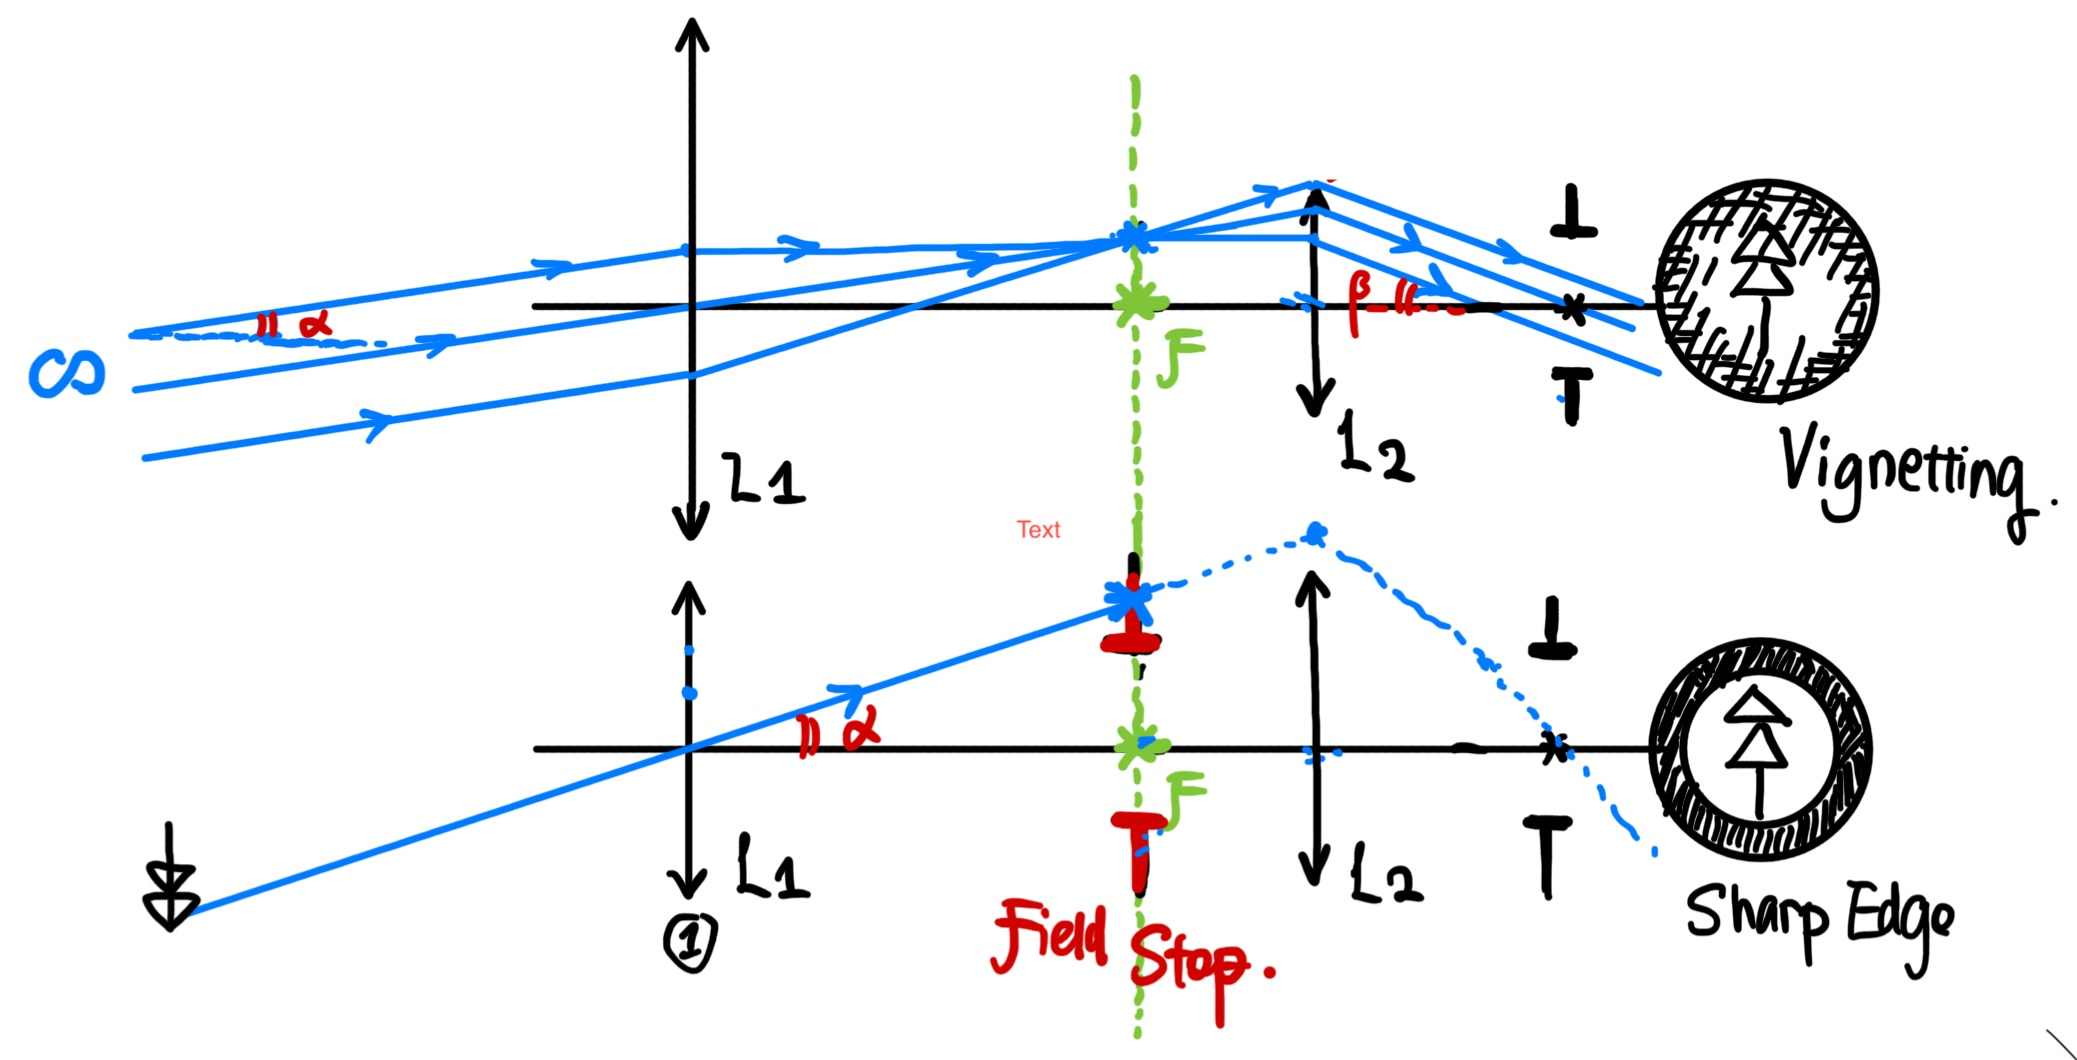
\includegraphics[width=0.8\textwidth]{Image/2_lens_ray_2.jpg}
    \caption{Ray Tracing of Telescope}
    \label{telescope}
\end{figure}
\par 而显微镜(microscope)系统仅在望远镜系统前添加了一块焦距极短的凸透镜将近处物体成一虚像。其后的透镜称为\textbf{tube lens}用以在目镜前成一实像。在物镜和tube lens间光线平行,可以添加极化镜片等调制。对显微镜,\textbf{线性放大率(linear magnification)}是主要参数。市售物镜通常以[160或200mm]tube lens组合标注放大率,可与目镜放大率相乘得到显微镜放大率。
\begin{note}[Depth of Field]
    首先考察物平面上离轴R光源的的边沿射线(图\ref{depth}蓝),发现其光路径长度变化为$R\sin{\alpha}$,则小于$\lambda/2$时形成干涉无法分辨,该距离R称为\textbf{衍射极限(resolution limit)}。显微镜研究中常定义\textbf{数值孔径(Numerical aperture)}$NA\triangleq n\sin{\alpha}$,n为介质折射率,空气中为1:
    \[R_{lim}\approx\frac{\lambda}{2NA}\]
    再考察轴上离中心d的光源(图\ref{depth}绿),沿轴射线和边沿射线同时变化,其差为$d(1-\cos{\alpha})$。设距离A.S.为L,孔径半径D,容易导出:
    \[d\leq\frac{\lambda L^2}{D^2}\]
    两倍的d称为\textbf{景深(depth of field)},即可以清晰成像的纵深距离。也常写作:
    \[DOF\approx2.4\frac{\lambda L^2}{D^2}\]
    另一边,即像空间的纵深称为\textbf{焦深(depth of focus)},只需将L改成f,或写作
    \[DOF^*\approx2.4\lambda(f/\#)^2\]
    其中$f/\#\triangleq f/D$是摄影中常用的镜头参数,称\textbf{焦比(focal ratio)},无量纲。其倒数称为\textbf{相对孔径(relative aperture)},其平方与进光的辐照密度正比。
\end{note}
\begin{figure}[t] 
    \centering
    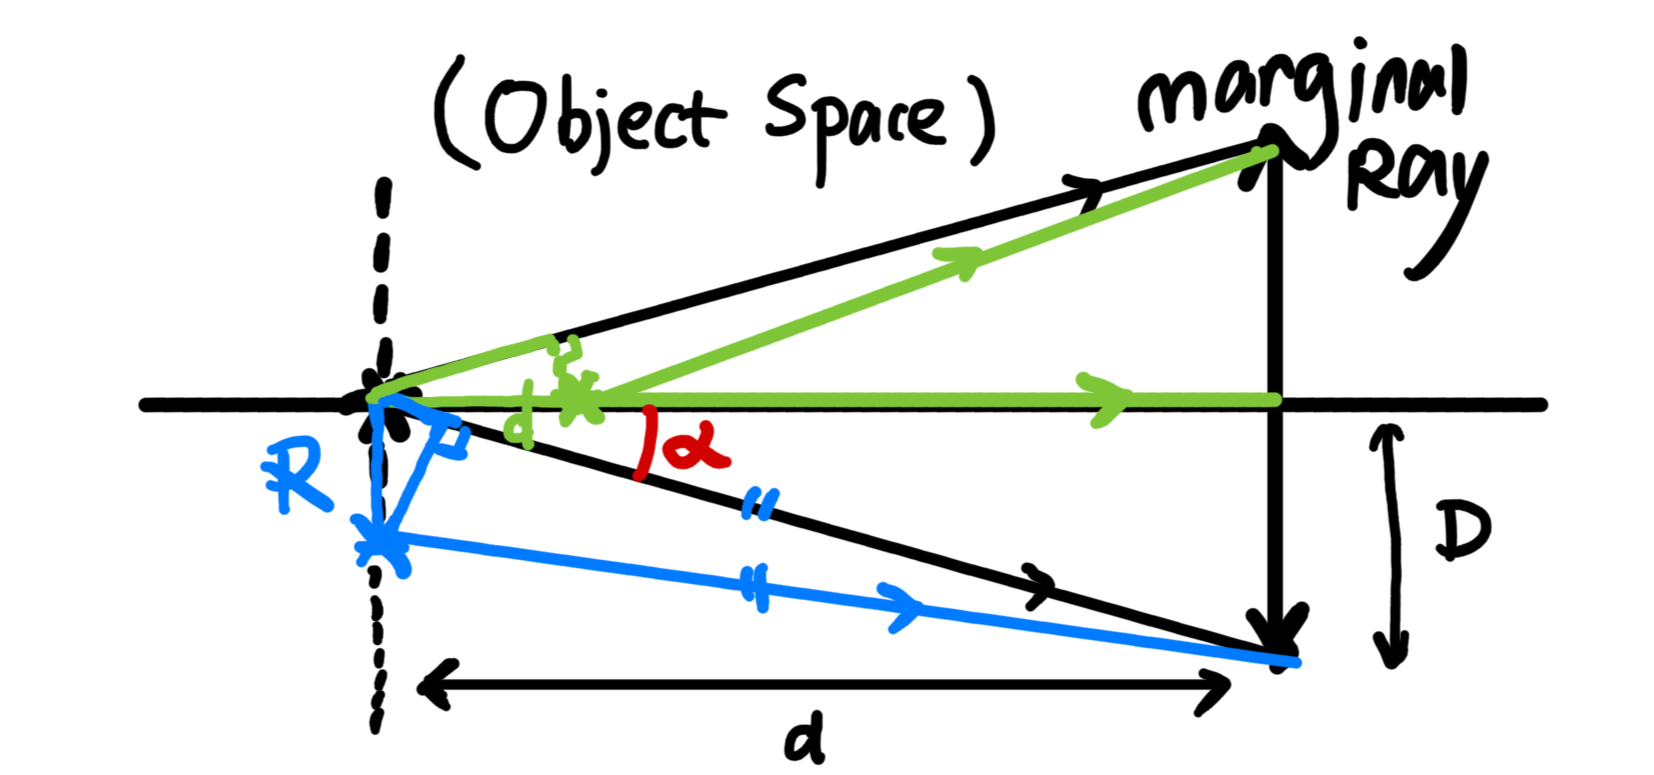
\includegraphics[width=0.5\textwidth]{Image/2_depth.jpeg}
    \caption{Radius and Depth of Imaging}\label{depth}
\end{figure}
\par 正常显微镜在对离轴、焦内物体成像时,其放大率和位置都会偏移。\textbf{远心镜(Telecentric Microscope)}通过在物镜焦距处添加额外孔径来限制焦内离轴光的线路,使之与焦面光产生的光锥形状一致。其成像没有透视关系,各距离物体放大率相等,适合进行距离测量。其光路见图\ref{tele}。
\begin{figure}[b] %two figures
    \centering
    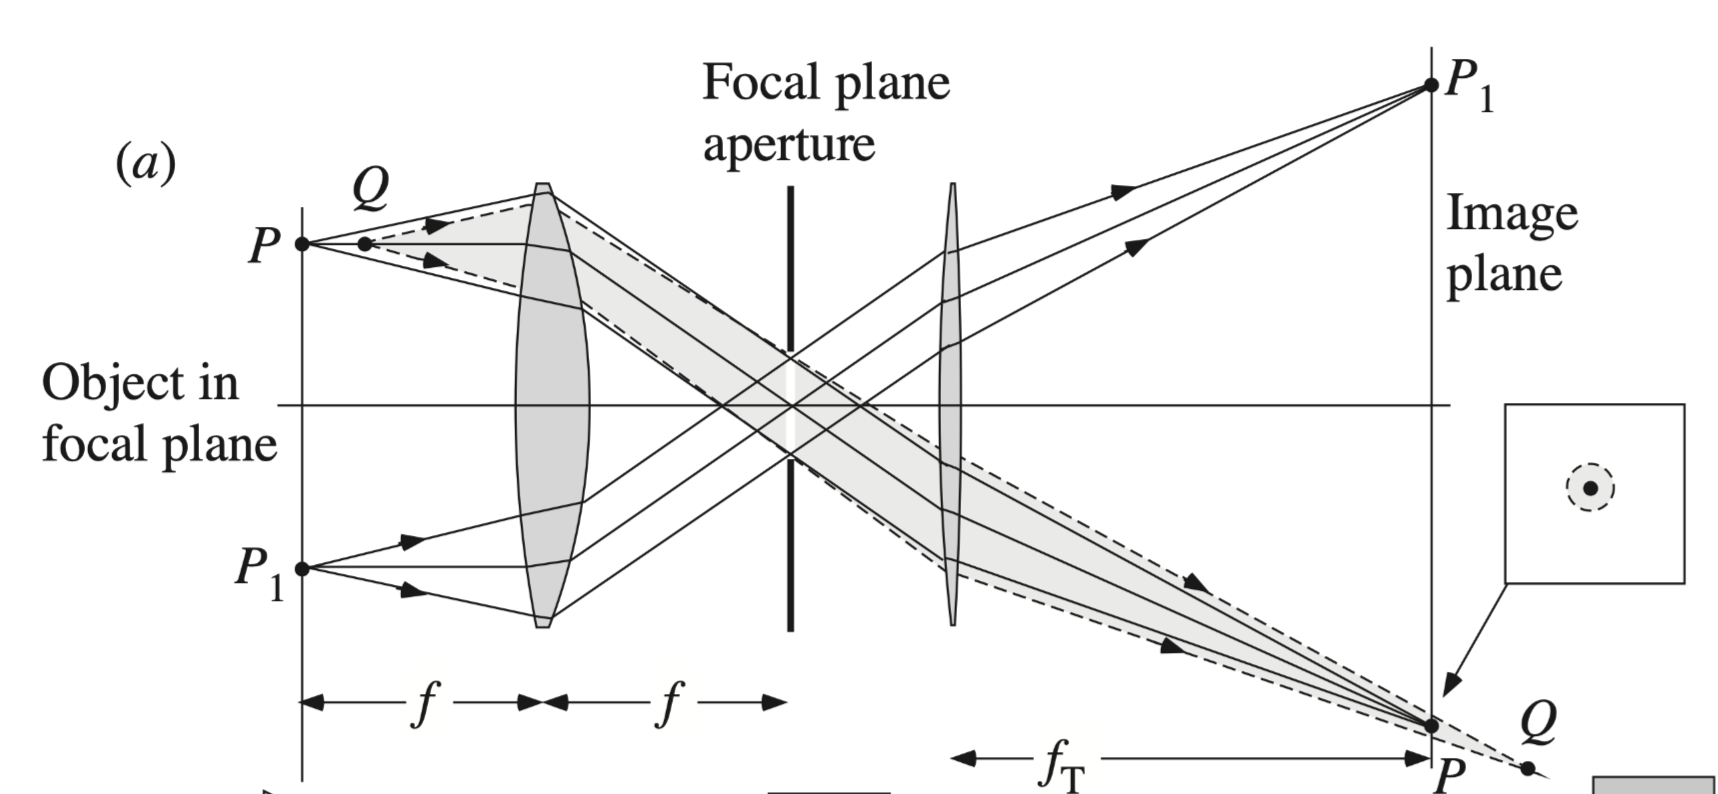
\includegraphics[width=0.65\textwidth]{Image/2_tele.png}
    \caption{Rays of Telecentric Microscope}
    \label{tele}
\end{figure}
\section*{基于矩阵的几何光学}
前面的讨论基于薄透镜的近似。为了处理更复杂的体系,我们考虑分析的方法。由于我们的体系关于z轴对称,只要指定了距离z的距离$y$和同z轴的角度$\theta$即可确定任一条近轴的光线点。记某点所在介质为n1,用列向量表示为$(y,n_1\theta)^T$.则在均匀介质中其传播距离t的转移矩阵T为:
\begin{equation}
    T=\begin{pmatrix}
        1 & t/n_1 \\
        0 & 1
    \end{pmatrix}
\end{equation}
其构造即高度变化而角度(第二行)不变。而在界面处的折射亦可用一个转移矩阵R描述:
\begin{equation}
    R=\begin{pmatrix}
        1 & 0 \\
        \frac{n_1-n_2}{R} & 1
    \end{pmatrix}
\end{equation}
同理,高度保持不变而角度发生变化(射入透镜时角度变小)。两个操作结合以描述1点经过折射传播到2点的矩阵:
\begin{equation}
    M_{21}=RT
\end{equation}
注意到R和T点行列式都是1,因为透镜体系中所有操作都可以由这两种矩阵组合而成,转移矩阵都有单位行列式。
\subsection*{透镜的矩阵表示}
考虑一个由两个曲面构成的凸透镜,曲面间距为t,折射率为n。两边介质折射率为1,则其转移矩阵可算出:
\begin{equation}
    M_{21}=\left(\begin{array}{cc}
        1+\frac{t(1-n)}{n R_{1}} & t / n \\
        (n-1)\left(\frac{1}{R_{2}}-\frac{1}{R_{1}}\right)-\frac{t(1-n)^{2}}{R_{1} R_{2} n} & 1+\frac{(n-1) t}{R_{2} n}
        \end{array}\right)
        \label{M21}
\end{equation}
当t远小于凸面半径时,化简为:(f与式(\ref{f})定义一致)
\begin{equation}
    M_{21}=\begin{pmatrix}
        1 & 0 \\
        (n-1)\left(\frac{1}{R_{2}}-\frac{1}{R_{1}}\right) & 1
    \end{pmatrix}=\begin{pmatrix}
        1 & 0 \\
        -1/f & 1
    \end{pmatrix}
\end{equation}
当两边介质不同时:
\begin{equation}
    M_{21}=\begin{pmatrix}
        1 & 0 \\
        \frac{n-n_2}{R_2}-\frac{n_1-n}{R_1} & 1
    \end{pmatrix}
\end{equation}
当两个凸面半径相同时,焦距是无穷,但应当代入完整的展开式(\ref{M21})计算。
\par 当多个镜片构成镜组时,其实体总是被左右两边的\textbf{顶点(vertice)} $V_1,V_2$限制。称其左右边为\textbf{物空间(object space)}和\textbf{像空间(image space)}。则在物空间总出现虚像,像空间出现实像。这对概念将助于接下来对成像的讨论。
\subsection*{成像过程的矩阵表示}
设事件平面内有从($z_O$,y1)以$\theta$发射的光线,其在$z_I$点的状态可以由中间体系的矩阵$M_{21}$完全表达:
\begin{equation}
    \begin{pmatrix}
        y_2\\
        n_2\theta_2
    \end{pmatrix}=\begin{pmatrix}
        A & B \\
        C & D
    \end{pmatrix}\begin{pmatrix}
        y_1\\
        n_1\theta_1
    \end{pmatrix}
\end{equation}
然而,若要求成像,那么该点发出的任意角度光线应也在$y_2$点,即算得的$y_2$应与角度无关,也就是B=0。$M_{21}$显然和物距相距相关,故$z_O$-$z_I$关系可以从中解出。此时称两点$z_O,z_I$所在平面称为\textbf{共轭面(conjugate planes)}。因为汇聚一点,易算出线性放大率(利用B=0):
\begin{equation}
    M_L=\frac{y_2}{y_1}=A
\end{equation}
\begin{figure}[t] %two figures
    \centering
    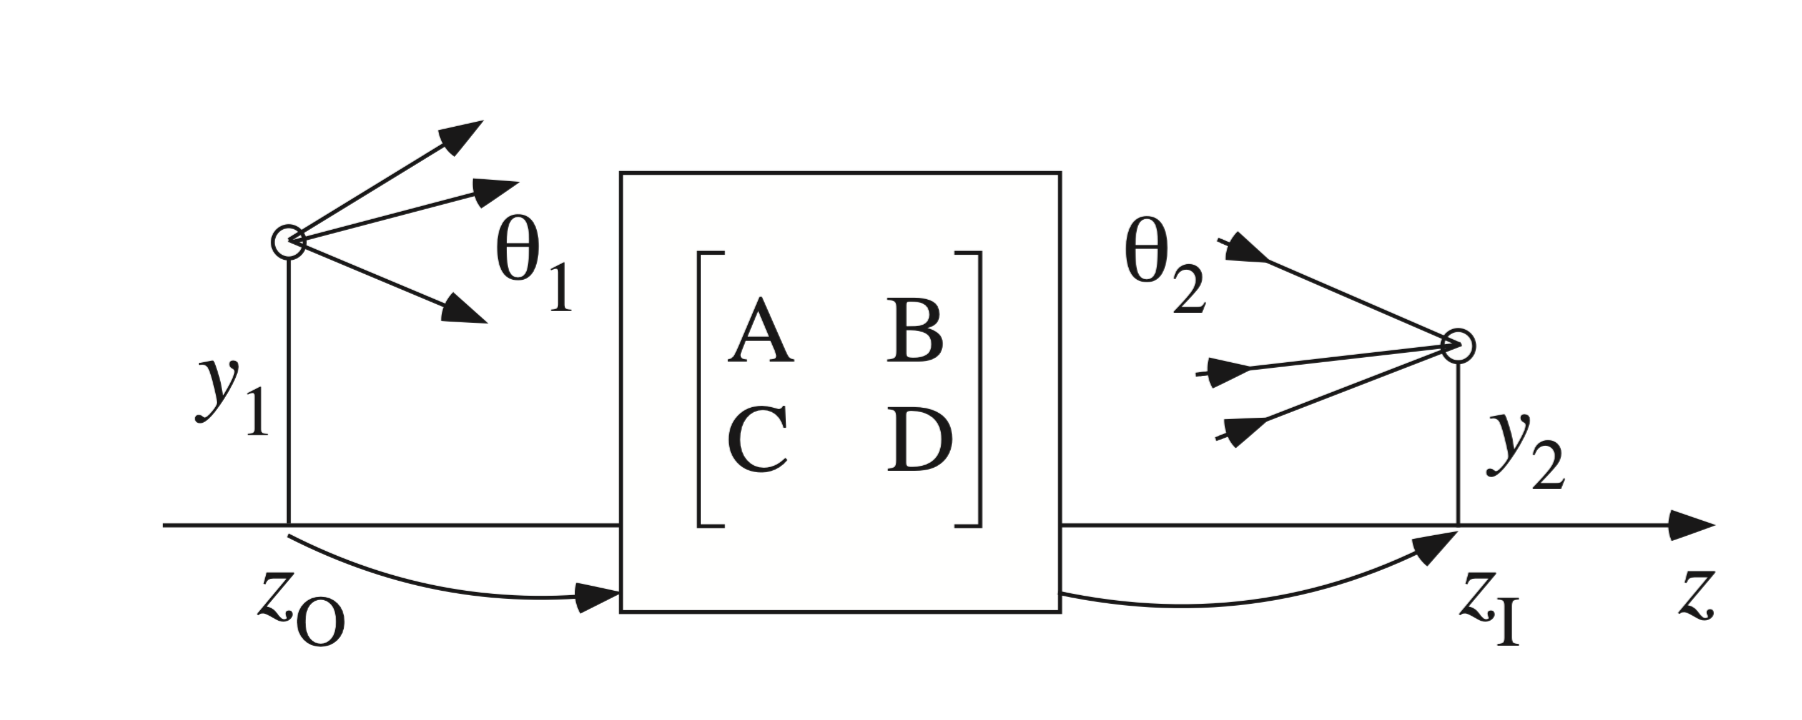
\includegraphics[width=0.7\textwidth]{Image/2_Matrix.png}
    \caption{Matrix Method for Imaging}
    \label{Matrix}
\end{figure}
同样易算出角放大率(令$y_1$=0,利用AD=1):
\begin{equation}
    M_A=\frac{\theta_2}{\theta_1}=\frac{Dn_1\theta_1}{n_2\theta_1}=D\frac{n_1}{n_2}=\frac{1}{M_L}\frac{n_1}{n_2}
\end{equation}
\par 考虑薄透镜的1到2点转移矩阵:
\begin{equation}
    M_{21}=\begin{pmatrix}
        1-v/f & -u+v+vu/f \\
        -1/f & 1+u/f
    \end{pmatrix}
\end{equation}
故令B=0,容易给出透镜制作公式 \ref{lens}。此外,利用AD=1可以导出如下公式:
\begin{theorem}[Newton's Equation]\label{Newton}
    \[(f+u)(f-v)=f^2\]
\end{theorem}
注意该式仅需要物、像与焦点的相对位置,而不需要明确V1,V2。因而在薄透镜体系外也广泛适用。
\par 当转移矩阵中C=0时,出射角度同入射高度无关,即平行光仍会是平行光,但角度不同。这类系统称为\textbf{无焦系统(afocal/telescopic)},平行光在无穷远处成虚像。
\subsection*{基点和基面}
\begin{figure}[t] %two figures
    \centering
    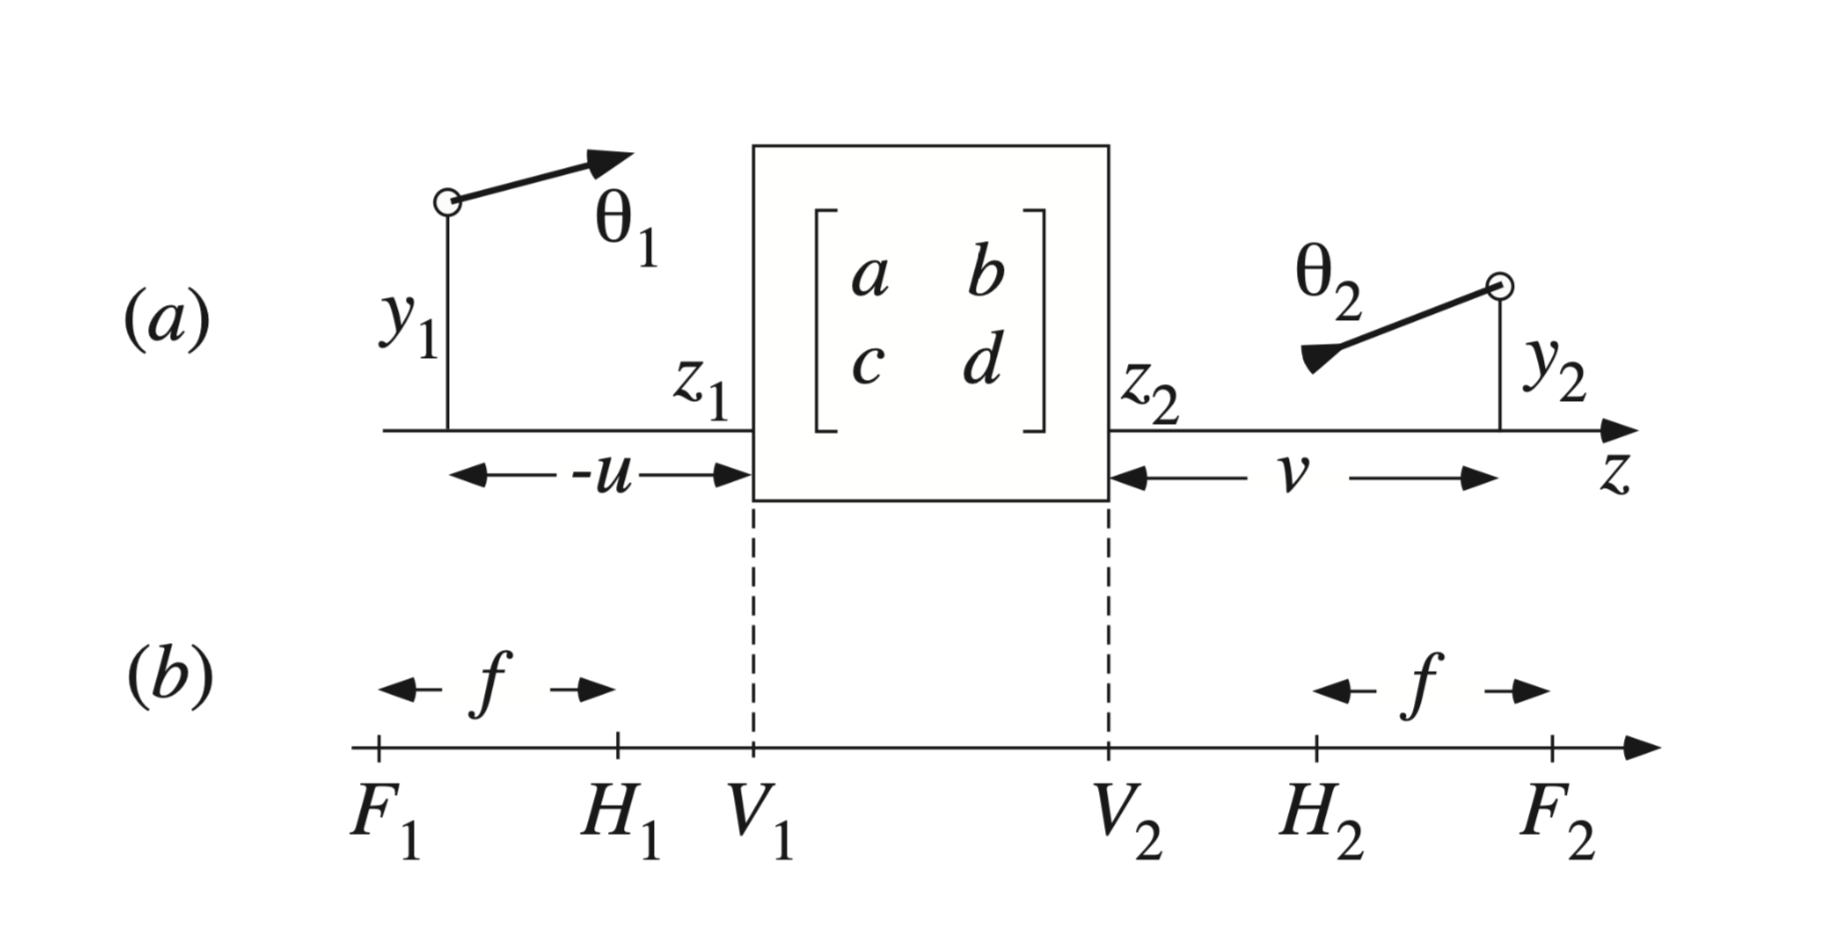
\includegraphics[width=0.7\textwidth]{Image/2_Matrix2.png}
    \caption{Matrix Method for General System}
    \label{Matrix2}
\end{figure}
为了发展一套适用于任何镜组系统的模型,我们将薄透镜的矩阵替换为小写字母的矩阵,并引入V1,V2两个顶面(坐标$z_1,z_2$)表示其占据的空间(见图\ref{Matrix2})。物距u和像距v都以之为基准。注意图\ref{Matrix}中大写字母阵表示O到I所有路程的转移矩阵,而小写字母矩阵仅代表V1到V2间的某特殊系统。因而不难算出总的转移矩阵形式(两边介质折射率为1):
\begin{equation}
    \begin{pmatrix}
        A & B \\
        C & D
    \end{pmatrix}=\begin{pmatrix}
        a+vc & b-au+vd-vcu \\
        c & d-cu
    \end{pmatrix}
\end{equation}
引入成像条件得到一下两个等式:
\begin{equation}
    b-au+vd-vcu=0
\end{equation}
\begin{equation}
    (a+vc)(d-cu)=1
\end{equation}
同公式\ref{Newton}比较发现,如定义$-1/c$为\textbf{等效焦距(effective focal length)} $f_{e}$则可得到相似的形式:
\begin{equation}
    (f_e-d/c+u+1/c)(f_e-a/c-v+1/c)=f_{e}^2
\end{equation}
定义\textbf{主平面(principle planes)} $\mathcal{H}_1,\mathcal{H}_2$坐标为:
\begin{equation}
    {H}_1=\frac{d-1}{c}+V_1=u_p+V_1
\end{equation}
\begin{equation}
    {H}_2=\frac{1-a}{c}+V_2=v_p+V_2
\end{equation}
则上式可代入物体到主平面距离以完全符合Newton方程的形式:
\begin{framed}
    \begin{equation}
        (f_e+(u-u_p))(f_e-(v-v_p))=f_{e}^2
    \end{equation}
\end{framed}
\noindent 进一步考察无穷远处的物和像不难得到与主平面间隔一个等效焦距$f_e$的\textbf{焦点}$F_1,F_2$坐标:
\begin{equation}
    F_1=d/c+V_1
\end{equation}
\begin{equation}
    F_2=-a/c+V_2
\end{equation}
\par 换言之,如果知道了主平面和等效焦距,那么V1-V2间的系统可以等效为一个薄透镜。其物-像公式中距离用以主平面为参考的距离代替。这四个点称为\textbf{基点(cardinal points)}。通过主平面的光必定以相同的位置射出,或言两主平面相互共轭且线性放大率为1。当两边折射率相同时,角放大率也是1,不然则可定义一组\textbf{节点(nodel points)} $N_1,N_2$,从之出发的光必定以相同的角度在另一点射出。根据这六个点可以描述任一系统。普遍的形式如下给出:
\begin{equation}
    {H}_{1/2}=\frac{d-1}{c}n_1[or \frac{1-a}{c}n_2]+V_{1/2}
\end{equation}
\begin{equation}
    {N}_{1/2}=\frac{n_1-n_2a}{c}[or \frac{n_1d-n_2}{c}]+V_{1/2}
\end{equation}
\par 用基点的概念可简化照相机的模型。长焦系统中,凸透镜和凹透镜的组合让两个主平面都处于机身左侧,从而使较长的有效焦距仍能聚焦在cmos上。见图\ref{camera}。
\begin{figure}[t] %two figures
    \centering
    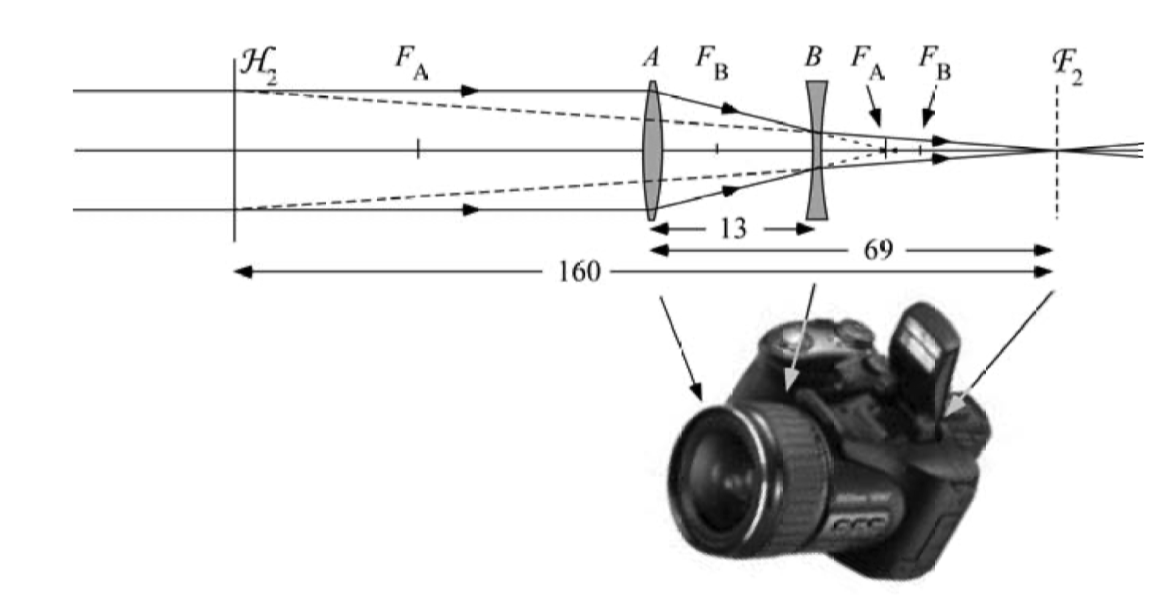
\includegraphics[width=0.7\textwidth]{Image/2_Camera.png}
    \caption{Cardinal Points of Camera}
    \label{camera}
\end{figure}
\section*{畸变}
在
\end{document}
